\section{Règles} % (fold)
\label{rules}

\subsection{La carte} % (fold)
L'arène (ou tout simplement la carte) est un tableau à deux dimensions (autrement dit, un rectangle).
Ce rectangle est indexé de \lstinline!(0,0)! à (\heightmax,\widthmax).

\begin{center}
    \begin{tabular}{|c|c|c|c|}
        \hline
            (0,0) & \dots & \dots & (0,\widthmax) \\
        \hline
            &  &  &  \\
        \hline
            &  &  &  \\
        \hline
            (\heightmax,0) & \dots & \dots & (\heightmax,\widthmax) \\
        \hline

    \end{tabular}
\end{center}

Chaque case du tableau représente le sol de l'arène ; dans notre cas, il s'agit soit de \ground{} (où les entités peuvent se déplacer) ou de \water{} (où les entités ne peuvent se déplacer).
Une seule entité par case est permise.

% subsection La carte (end)

\subsection{Les entités du jeu} % (fold)

Dans cette partie sont présentées les entités du jeu.
Une entité est une unité capable de se mouvoir au cours de la partie.
Un mouvement peut se faire vers le haut (\north{}), vers le bas (\south{}), vers la droite (\east{}) ou vers la gauche (\west{}).
Une entité peut se déplacer de \movelen{} cases par tour (dans notre cas, \movelen{}=1).

\begin{figure}[htbp]
    \centering
    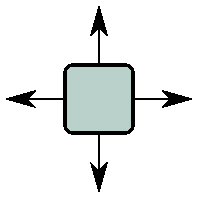
\includegraphics[width=0.2\textwidth]{pics/entite_move}
    \caption{Mouvement autorisé d'une entité}
    \label{move}
\end{figure}

Une entité est soit contrôlée par un joueur ou par l'ordinateur (les humains par exemple).
Chaque entité à un rayon de vision \viewradius{} (commun pour toutes les entités) fixé au début d'une partie.

\begin{figure}[htbp]
    \centering
    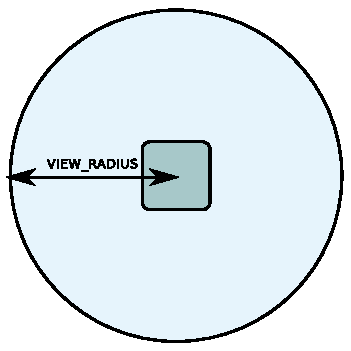
\includegraphics[width=0.4\textwidth]{pics/entite_view}
    \caption{Vision d'une entité}
    \label{view}
\end{figure}

\subsubsection{Les humains} % (fold)
Les humains sont les entités ressources de ce jeu.
Ils sont contrôlés par l'ordinateur et ont un comportement plus ou moins évolué.
Ils n'ont pas de capacité spéciale et tentent d'éviter de se faire contaminer.


% subsubsection Les humains (end)

\subsubsection{Les policiers} % (fold)
Les policiers sont des humains équipés d'une arme à feu.
De ce fait, ils sont capables de tuer les zombies autour d'eux.
Toutefois, leur nombre de balles est limité et ils commencent avec \bulletamount{} balles au début d'une partie.
Une fois que leur stock de balles est épuisé, ils redeviennent de simples humains.

Lorsqu'un zombie est à portée de tir, c'est à dire à une distance inférieure à \shotradius{}, le policier tire automatiquement sur le zombie.
Le tir a une probabilité de chance de réussite de \shotsuccess{}.
Lorsqu'il y a plusieurs zombies à portée, le choix de la cible est aléatoire.

Un policier peut se faire contaminer par un zombie.
Dans ce cas de figure, en plus de la capacité de contaminer des humains, le zombie policier peut tirer sur des zombies adverses.
Comme pour le policier, le tir est automatique et aléatoire si plusieurs zombies sont à portée.

Lorsque le zombie n'a plus de balles, il redevient un zombie comme les autres.


% subsubsection Les policiers (end)

\subsubsection{Les zombies} % (fold)
Les zombies sont les unités que vous controlez.
Elles peuvent\footnote{doivent} contaminer les humains et étendre leur contrôle sur la carte.
Pour cela, chaque zombie dispose d'un compteur de contagions, initialisé à sa création à \contagionamount.
À chaque contagion, ce compteur est décrémenté, ce qui influe sur la prochaine contagion (cf \ref{contagion}).


% subsubsection Les zombies (end)

\subsubsection{Les berzerks} % (fold)
Lorsqu'une contagion ne se passe pas comme désirée (cf \ref{contagion}), l'humain ciblé peut soit mourir, soit devenir un zombie incontrôlable, appelé berzerk.
Un tel zombie est contrôlé par l'ordinateur et ne peut être tué par un policier ou un zombie.
Par contre, il tue zombies et humains autour de lui, lorsqu'il explose, \berzerkdelay{} tours après sa création.
Son explosion tue toutes les entités autour de lui à une distance \berzerkradius{}.

% subsubsection Les berzerks (end)

% subsection Les entités du jeu (end)

\subsection{Les actions du jeu} % (fold)
Une entité (qu'elle soit contrôlée par un joueur ou non) peut se mouvoir dans la carte.
Tous les mouvements ne sont cependant pas possibles. Par exemple, se déplacer vers une case \water.

D'autre part, si deux entités (quelconques) se retrouvent sur la même case à la fin d'un tour, les deux meurent.

% subsection Les actions du jeu (end)

\subsection{Le déroulement d'une partie} % (fold)

Une partie est divisée en plusieurs phases.
Tout d'abord, une phase initiale, où toutes les informations statiques et fixées vous sont fournies.
Ensuite, vient le jeu au tour par tour.

Au début de chaque tour, le joueur a connaissance de :
\begin{itemize}
    \item la position de nouvelles cases de type \water{} découvertes ;
    \item la position des entités, leur type et leur équipe ;
    \item la liste des zombies policiers du joueur qui ont réussi à abattre un autre zombie ;
    \item la liste des zombies du joueur nouvellement créés et quels zombies les ont créés.
\end{itemize}

Le brouillard de guerre s'applique de manière invisible pour le joueur.
On ne lui transmet que les informations qu'il est capable de percevoir.
Une fois qu'un joueur a reçu toutes ces informations, il est capable de décider quelle action fait chacune de ses entités.
Une fois que ce choix est réalisé, on peut exécuter un tour de jeu.


Un tour consiste en la succession d'étapes :

\begin{enumerate}
    \item Déplacer les entités ;
    \item Actions automatiques (tir, explosion berzerk, etc.) ;
    \item Gestion des attaques ;
    \item Gestion des contaminations.
\end{enumerate}

À la fin de chaque tour, on vérifie que les conditions de victoires et de défaites ne sont pas atteintes.
Un joueur est considéré vaincu lorsqu'il n'a plus d'entités sur la carte, que son programme s'est interrompu ou qu'il ne répond plus dans les délais.
Un joueur est considéré vainqueur lorsqu'il est le dernier sur la carte.

Le jeu se termine lorsque un joueur est déclaré vainqueur ou que \turnmax{} tours se sont déroulés (dans ce cas, le score permet de déterminer le vainqueur).

% subsection Le déroulement d'une partie (end)

\subsection{Score d'une partie} % (fold)
Au cours d'une partie, un joueur peut gagner ou perdre des points.
Voici les événements qui influent sur les scores :
\begin{itemize}
    \item Perte d'un zombie = -1 points ;
    \item Humain contaminé = 2 point ;
    \item Zombie tué = 3 point ;
    \item Policier tué = 5 points.
\end{itemize}

% subsection Score d'une partie (end)

\subsection{Contamination d'un humain} % (fold)
\label{contagion}
Lorsqu'un zombie est proche d'un humain (dans un rayon de distance \contagionradius{}), il a des chances de contaminer cet humain.
Dans ce cas de figure, on calcule les probabilités de contamination de la manière suivante :\\
    $$n = \text{compteur de contagions du zombie}$$
    $$P_{contagion} = \frac{n}{\contagionamount}$$

En cas de succès, un nouveau zombie (possiblement policier) est créé et affecté à l'équipe contaminante.
Autrement, l'humain peut soit mourrir soit devenir un berzerk.
La probabilité de créer un berzerk est calculée de la manière suivante :\\
    $$n = \text{compteur de contagions du zombie}$$
    $$P_{berzerk} = \frac{\contagionamount - n}{\contagionamount} * \frac{1}{4}$$

Si plusieurs zombies se situent dans le rayon de contagion d'un humain, on choisit l'équipe la plus représentée puis le zombie ayant un compteur de contagions le plus élevé de cette équipe.
En cas de représentation égale (des équipes) ou de compteurs égaux pour plusieurs zombies, on utilise de l'aléatoire pour choisir l'équipe et/ou le zombie.
Puis les calculs ci-dessus sont réalisés.

Si plusieurs humains se situent autour d'un zombie, l'algorithme ci-dessus est joué pour chacun de ces humains.


% subsection Contamination d'un humain (end)

\subsection{Résolution de combats} % (fold)

Lorsque plusieurs zombies d'équipes différentes sont situés à une distance inférieure ou égale à \attackradius{}, voici comment est déterminé si un zombie est en vie ou non :

\begin{lstlisting}[caption=Résolution de combats, columns=fullflexible]
for every zombie:
        for each enemy in range of zombie:
            if (enemies_in_range(zombie)) >= (enemies_in_range(enemy)) then
                the zombie is marked dead
                /* actual removal is done after all battles are resolved */
                break
    
\end{lstlisting}

% subsection R (end)

\subsection{Distances} % (fold)

Vous avez besoin de manipuler des distances au cours du projet (notamment pour les rayons d'actions).
Dans ce projet, on se basera exclusivement sur la distance euclidienne\footnote{http://en.wikipedia.org/wiki/Euclidean\_distance}.

La distance entre deux points est calculée de la manière suivante :
\begin{center}
    $$ d(p,q) = \sqrt{(p_x - q_x)^2 + (p_y - q_y)^2} $$
    
\end{center}

% subsubsection Distances (end)

\subsection{Disqualification} % (fold)

Un joueur peut être disqualifié pour différentes raisons :
\begin{itemize}
    \item son programme a planté ;
    \item il ne répond plus dans les délais de manière répêtée ;
    \item le programme tente de faire une action jugée illégale.
\end{itemize}

Lorsqu'un joueur est disqualifié, ses entités restent présentes sur la carte mais restent immobiles jusqu'à la fin de la partie (ou leur disparition).

% subsection Disqualification (end)

\subsection{Temps de réponse} % (fold)

À chaque tour, vous avez un temps limite pour choisir les actions de vos entités.
\timinglimit{} désigne cette limite ; elle est fixée au début d'une partie et est valide tout au long d'une partie.

% subsection Temps de réponse (end)

\subsection{Valeurs fixées} % (fold)

Certaines données ont peu de chance de changer entre plusieurs parties.
Elles sont tout de même données en début de parties.
Les voici :

\begin{itemize}
    \item \movelen{} = 1 ;
    \item \viewradius{} = ? ;
    \item \bulletamount{} = 9 ;
    \item \shotradius{} = ? ;
    \item \shotsuccess{} = 50 ;
    \item \contagionamount{} = 9 ;
    \item \contagionradius{} = ? ;
    \item \berzerkdelay{} = 5 ;
    \item \berzerkradius{} = ? ;
    \item \attackradius{} = ? ;
    \item \timinglimit{} = 500ms.
\end{itemize}
% subsection Valeurs fixées (end)


% section Règles (end)
